Un matériau n'est pas critique seulement parce qu'il est rare. (\cite{geldron_lepuisement_2017}) différencie justement plusieurs types de métaux. D'abord, les métaux rares et très rares sont catégorisés par leur concentration dans la croûte terrestre qui est comprise entre 1 et 1000 ppm pour les premiers (cuivre, nickel, cobalt...), et inférieure à 1 ppm pour les seconds (platinoïdes...). Les petits métaux sont classés ainsi du fait des faibles volumes produits et de la taille du marché. Les métaux dits stratégiques sont considérés comme tels par des entreprises, des Etats, ou par des secteurs, selon le degré de leur dépendance. Enfin, les métaux critiques le sont du fait d'un épisode d'embargo, ou de menaces émises par un pays producteur.
\smallbreak
La criticité est communément déterminée selon deux critères. Premièrement, elle l'est à partir de l'évaluation du risque d'approvisionnement, qui se caractérise par des aspects techniques, économiques, régulatoires et politiques. Secondement, la vulnérabilité à la restriction des approvisionnements est examinée, c'est-à-dire les conséquences économiques d'une baisse, la substituabilité du métal, et son importance stratégique (\cite{hatayama_adopting_2018}). Par exemple, en France, c'est cette méthodologie d'évaluation qui est appliquée. Le Comité pour les métaux stratégiques mesure le risque d'approvisionnement à travers une cartographie des flux de la chaîne d'approvisionnement, de l'extraction à la production de métal. Quant à la vulnérabilité au risque susnommé, elle est estimée à partir d'échanges avec les fédérations professionnelles et les acteurs industriels (\cite{comes_note_2018}). 
\smallbreak
Ces deux critères sont aussi les axes des matrices d'évaluation des risques, soit la probabilité d'occurence d'un risque, et la sévérité des conséquences en cas de réalisation. La première de ces matrices a été établie en 2008 aux Etats-Unis (\cite{hache_vers_2019}). Il faut donc mettre en avant le lien entre la mesure de la criticité et la recherche du maintien de la puissance. Cela passe aujourd'hui par la maîtrise des technologies de pointe, très dépendantes de la disponibilité de multiples métaux, expliquant ainsi leur caractère stratégique.
\smallbreak
(\cite{hache_vers_2019}) complètent ces définitions des matériaux critiques. Ces derniers sont utiles à de multiples secteurs de l'industrie, sont peu substituables, leurs usages industriels croissent dans le temps, leur potentiel de recyclage est limité, leur valeur économique est élevée, leur production et leurs réserves sont concentrées géographiquement et les produire peut engendrer des externalités négatives sur l'environnement (voir figure \ref{fig:criticite}).
\begin{figure}
    \centering
    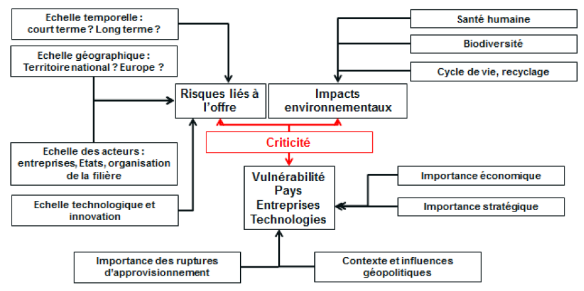
\includegraphics[width=0.8\textwidth]{Images/02 appro/schema criticite.png}
    \caption{Evaluer la criticité des matières premières. Source : \cite{hache_vers_2019}}
    \label{fig:criticite}
\end{figure}
Les auteurs font état d'une multiplicité d'indicateurs utilisés dans la littérature pour mesurer la criticité, qu'ils classent, conformément à la définition citée au paragraphe précédent, entre ceux relatifs à la vulnérabilité économique et ceux rattachés aux risques sur l'offre, sachant que certains peuvent appartenir aux deux groupes. Les premiers peuvent être ordonnés dans les sous groupes suivants : mesure de la dépendance (importance stratégique, dépendance aux importations, volume de la consommation...), valeur économique (valeur des produits affectés, valeur des matériaux utilisés) et substituabilité et recyclage (recyclabilité du produit, existence d'un substitut, capacité à innover...). Quant aux seconds, ils peuvent être groupés ainsi : indicateurs géologiques et physiques (dépendance aux coproduits, présence dans la croûte terrestre, vulnérabilité au changement climatique...), indicateurs économiques et financiers (investissements dans le secteur minier, volatilité des prix des matières premières, existence d'un marché financier...), indicateurs stratégiques (concentration par pays et des entreprises, risque d'embargo...) et enfin substituabilité et recyclage (potentiel de recyclage, existence d'un substitut). En outre, il existe actuellement une discussion dans la communauté scientifique autour de l'ajout d'un troisième axe dans l'évaluation de la cricité : les conséquences environnementales de la production d'un matériau. Cela pose en effet la question de l'indépendance des enjeux qui en découlent par rapport aux ruptures d'approvisionnement et à la vulnérabilité économique.
\smallbreak
Dans l'ensemble, il ressort de la littérature que la criticité est une notion complexe, dont la pluridisciplinarité des approches et la multiplicité des horizons temporels choisis rend difficile la comparaison entre études. Dès les années 1970, le débat sur la déplétion des ressources subvenu entre les auteurs du rapport \textit{The Limits to Growth} issus de la dynamique des systèmes et des économistes, dont Friedrich Hayek, en est la preuve. (\cite{tilton_assessing_2003}) s'est appuyé sur cette controverse pour formuler l'existence de deux paradigmes. D'abord, il énonce celui des géologues raisonnant à partir de stocks non-renouvelables de ressources et considérant les limites de ceux-ci face à une demande grandissante dans le temps. Il le compare au paradigme des économistes, qui fondent leur réflexion sur la notion de coût d'opportunité. Dans cette approche, l'accent est plus mis sur les substituts, le recyclage, et l'élasticité-prix de la demande. Si les géologues prennent en compte le très long terme, les économistes réfléchissent avec le temps des cycles économiques, c'est-à-dire les court et moyen termes. Pour Tilton, la déplétion économique due à un effondrement de la demande face à une hausse des prix des matières premières est plus envisageable qu'une déplétion géologique. (\cite{hache_vers_2019}) notent toutefois que cet auteur n'a pas théorisé ces paradigmes dans le cadre de la transition énergétique.

